
%%%%%%%%%%%%%%%%%%%%%%% file typeinst.tex %%%%%%%%%%%%%%%%%%%%%%%%%
%
% This is the LaTeX source for the instructions to authors using
% the LaTeX document class 'llncs.cls' for contributions to
% the Lecture Notes in Computer Sciences series.
% http://www.springer.com/lncs       Springer Heidelberg 2006/05/04
%
% It may be used as a template for your own input - copy it
% to a new file with a new name and use it as the basis
% for your article.
%
% NB: the document class 'llncs' has its own and detailed documentation, see
% ftp://ftp.springer.de/data/pubftp/pub/tex/latex/llncs/latex2e/llncsdoc.pdf
%
%%%%%%%%%%%%%%%%%%%%%%%%%%%%%%%%%%%%%%%%%%%%%%%%%%%%%%%%%%%%%%%%%%%

\let\origvec\vec
\documentclass[runningheads,a4paper]{llncs}



%******Figure and Table Package
\usepackage{color}
\usepackage{amsfonts}
%\usepackage{ulem}    % underline/strikethrough/wave lines
\usepackage{graphicx}  % figures
\usepackage{tabularx}
\usepackage{subfigure}
\usepackage{graphicx}
\usepackage{caption}
%\usepackage{subcaption}
\usepackage{multirow}
\usepackage{tikz}
\usetikzlibrary{shapes,shadows,calc}
\usepgflibrary{arrows}

\newcommand{\A}{\mathcal{A}}
\newcommand{\K}{\mathcal{K}}
\newcommand{\M}{\mathcal{M}}
\newcommand{\T}{\mathcal{T}}


\tikzset{
	sshadow/.style={opacity=.25, shadow xshift=0.05, shadow yshift=-0.06},
}

%-----#1 size, #2 angle, #3 aspect, #4 label next to the diamond
%-----#5 name of the node, #6 coordinate, #7 label
\def\schemel[#1,#2,#3,#4,#5,#6]#7{ %
	\node[draw, diamond, shape aspect=#3, rotate=#2, minimum size=#1, %
	bottom color=green!55, top color=green!25, color=green!65!black, %
	drop shadow={sshadow,color=green!60!black}, #4] (#5) at #6
	{\textcolor{green!40}{bla}}; %
	\node at #6 {#7};%
}

\def\schemer[#1,#2,#3,#4,#5,#6]#7{ %
	\node[draw, diamond, shape aspect=#3, rotate=#2, minimum size=#1, %
	bottom color=green!65, top color=green!30, color=green!60!black, %
	drop shadow={sshadow,color=green!65!black}, #4] (#5) at #6
	{\textcolor{green!53}{bla}}; %
	\node at #6 {#7}; %
}

%-----TBoxes
%-----#1 height, #2 width, #3 anchor for the label, #4 name of the node, #5
%-----coordinate, #6 label
\def\tboxl[#1,#2,#3,#4,#5]#6{%
	\node[draw, drop shadow={opacity=.35}, minimum height=#1, minimum width=#2, %
	inner color=blue!45, outer color=blue!55, color=blue!40!black] (#4) at #5 {}; %
	\node[anchor=#3,inner sep=2pt] at (#4.#3) {#6};%
}

\def\tboxr[#1,#2,#3,#4,#5]#6{%
	\node[draw, drop shadow={opacity=.35}, minimum height=#1, minimum width=#2, %
	inner color=blue!35, outer color=blue!45, color=blue!50!black] (#4) at #5 {}; %
	\node[anchor=#3,inner sep=2pt] at (#4.#3) {#6}; %
}

%-----#1 name of the node, #2 coordinate, #3 label
\def\entity[#1,#2]#3;{
	\node[draw,drop shadow={opacity=.4,shadow xshift=0.04, shadow
		yshift=-0.04},color=blue!30!black,fill=white,rounded corners=3] (#1) at #2 {#3};
}

%-----#1 from node, #2 to node, #3 specification of a node (label), #4
%-----dashed, or other parameters for draw
\def\isaedge[#1,#2,#3,#4];{ 
	\draw[-triangle 60,color=black!20!black,#4,fill=white] (#1) -- #3
	(#2);  
}

%-----ABoxes
%-----#1 height, #2 width, #3 aspect, #4 name of the node, #5
%-----coordinate, #6 label
\def\aboxl[#1,#2,#3,#4,#5]#6{%
	\node[draw, cylinder, alias=cyl, shape border rotate=90, aspect=#3, %
	minimum height=#1, minimum width=#2, outer sep=-0.5\pgflinewidth, %
	color=orange!40!black, left color=orange!70, right color=orange!80, middle
	color=white] (#4) at #5 {};%
	\node at #5 {#6};%
	\fill [orange!30] let \p1 = ($(cyl.before top)!0.5!(cyl.after top)$), \p2 =
	(cyl.top), \p3 = (cyl.before top), \n1={veclen(\x3-\x1,\y3-\y1)},
	\n2={veclen(\x2-\x1,\y2-\y1)} in (\p1) ellipse (\n1 and \n2); }

\def\aboxr[#1,#2,#3,#4,#5]#6{%
	\node[draw, cylinder, alias=cyl, shape border rotate=90, aspect=#3, %
	minimum height=#1, minimum width=#2, outer sep=-0.5\pgflinewidth, %
	color=orange!50!black, left color=orange!50, right color=orange!60, middle
	color=white] (#4) at #5 {};%
	\node at #5 {#6};%
	\fill [orange!20] let \p1 = ($(cyl.before top)!0.5!(cyl.after top)$), \p2 =
	(cyl.top), \p3 = (cyl.before top), \n1={veclen(\x3-\x1,\y3-\y1)},
	\n2={veclen(\x2-\x1,\y2-\y1)} in (\p1) ellipse (\n1 and \n2); }

%-----#1 height, #2 width, #3 name of the node, #4
%-----coordinate, #5 label
\def\kbbox[#1,#2,#3,#4,#5]#6{
	\draw[dashed] node[draw,color=gray!50,minimum
	height=#1,minimum width=#2] (#4) at #5 {}; 
	\node[anchor=#3,inner sep=2pt] at (#4.#3)  {#6};
}

%-----#1 from node, #2 to node, #3 specification of a node (label), #4
%-----dashed, or other parameters for draw
\def\soledge[#1,#2,#3,#4];{
	\draw[dashed,-latex,#4] (#1) -- #3 (#2);
}



%**********Math package

\let\springervec\vec
\let\vec\origvec
\usepackage{amsmath}
\usepackage{amssymb}
\usepackage{latexsym}
\setcounter{tocdepth}{3}
\usepackage{graphicx}



%---Algorithm
\renewcommand{\thechapter}{\Roman{chapter}}
\renewcommand{\thesection}{\arabic{section}}

\usepackage[chapter]{algorithm}
\usepackage{algorithmicx}
\usepackage{algpseudocode}

\renewcommand{\thealgorithm}{\arabic{chapter}.\arabic{algorithm}} 


%----Graph
\usepackage{tikz,mathpazo}  % This package is used to draw the figure
\usetikzlibrary{shapes.geometric, arrows}
\usetikzlibrary{positioning,shapes.geometric}

\usepackage{palatino}
\usepackage{tikz}
\usetikzlibrary{shapes.geometric, arrows}
\usepackage{xcolor}
\usetikzlibrary{shapes,arrows,chains}

%----- pNet macros package
\usepackage{epsfig,enumitem}
\newcommand{\TODO}[1]{\textcolor{red}{\textbf{[TODO:#1]}}}
\newcommand{\NOTE}[1]{\textcolor{blue}{\textbf{[NOTE:#1]}}}
\newcommand{\ERIC}[1]{\textcolor{blue}{#1}}
\definecolor{darkgreen}{rgb}{0.1, 0.5, 0.1}
\newcommand{\coloncolon}{{:\hspace{-.2ex}:}}
\makeatletter
\newcommand{\raisemath}[1]{\mathpalette{\raisem@th{#1}}}
\newcommand{\raisem@th}[3]{\raisebox{#1}{$#2#3$}}
\makeatother

\usepackage{macrospNets}



\usepackage{url}


\urldef{\mailstu}\path|{tengfei.li}@stu.ecnu.edu.cn| 
\urldef{\mailecnu}\path|{jliu, hysun}@sei.ecnu.edu.cn|      
\newcommand{\keywords}[1]{\par\addvspace\baselineskip
\noindent\keywordname\enspace\ignorespaces#1}

\begin{document}

\mainmatter  % start of an individual contribution

% first the title is needed
\title{Model Checking for Open Concurrent Systems}

% a short form should be given in case it is too long for the running head
\titlerunning{Lecture Notes in Computer Science: Authors' Instructions}

% the name(s) of the author(s) follow(s) next
%
% NB: Chinese authors should write their first names(s) in front of
% their surnames. This ensures that the names appear correctly in
% the running heads and the author index.
%
\author{Tengfei Li
%\thanks{Corresponding author}%
\and Eric Madelaine \and *
}
%
\authorrunning{Lecture Notes in Computer Science: Authors' Instructions}
% (feature abused for this document to repeat the title also on left hand pages)

% the affiliations are given next; don't give your e-mail address unless you accept that it will be published


\institute{
%\mailstu\\
%\mailecnu\\
}

%
% NB: a more complex sample for affiliations and the mapping to the
% corresponding authors can be found in the file "llncs.dem"
% (search for the string "\mainmatter" where a contribution starts).
% "llncs.dem" accompanies the document class "llncs.cls".
%

\toctitle{Lecture Notes in Computer Science}
\tocauthor{Authors' Instructions}
\maketitle


\begin{abstract}

The verification of concurrent systems, especially concurrent systems with data, have been researched for many years. However, the composition of concurrent systems have not been solved well. The major problem is ...

\keywords{ pM$\mu$\quad $pMG $\quad pLTS }
\end{abstract}


\section{Introduction}
% no \IEEEPARstart

\section{Use-case: The BIP Failure-Timer architecture}
\TODO{Describe here the full Failure-Timer architecture, as taken from the Avocs paper, including an informal presentation of the original BIP system, its full translation into a pNet system (pLTSs and pNet nodes), and the generated Open Automaton}
\NOTE{All figures are already available from the Avocs paper sources.}

\section{Describing pLTS}


\subsection{pLTS}

In a pLTS, each state is composed of a set of $\mathit{state\ variables}$, and a transition is defined between two states. A triple with $\mathit{parameterised\ action}, \mathit{guard}$ and $\mathit{assignment}$ consists of the labelling function of the transition.

\subsubsection{Definition of pLTS}
We define pLTS as a triple: $pLTS\triangleq\ll S, s_{0}, \rightarrow \gg$ where:
\begin{itemize}
	\item $S$ is a set of states, and $s_{0}\in S$ is the initial state.
	\item $\rightarrow \subseteq S\times L\times S$ is the transition relation, with $L$ the set of labels of form $<\alpha, e_{b}, (x_{j} := e_{j})^{(j\in J)}>$, where $\alpha\in A_{V}$ is a parameterised action, $e_{b}\in B_{V}$ is a guard, and expression $E_{P}\cup A_{P}$ are assigned to $x_{j}$. If $s\xrightarrow{<\alpha, e_{b}, (x_{j}:=e_{j})^{j\in J}>}s' \in \rightarrow$, then $vars(e_{b})\subseteq vars(s)\cup vars(\alpha)$, and $\forall j\in J. vars(e_{j})\subseteq vars(s)\wedge x_{j}\in vars(s')$.
\end{itemize}


\begin{figure}
	\centering
	\begin{tikzpicture}[->, shorten >=2pt, >=stealth, node distance=3cm,
	noname/.style={ellipse, minimum width=5em, minimum height=3em,draw}]
	\node[noname] (1)                                             {$s_{0}$};
	\node[noname] (2) [right=of 1]                                {$s_{1}$};
	
	\path 	(1) edge [bend left]                  node[above] {$[true],\langle start?M\rangle,\{t:=M\}$} (2)
	(2) edge [bend left]                  node[below] {$[t=0], \langle timeout\rangle$} (1)
	(2) edge 			               node[above] {$\langle resume\rangle$} (1);
	\path[->] (2) edge [in=-10,out=20,loop] coordinate[pos=0.52] (midp) node[right] {$[t>0], \langle tick\rangle, \{t:=t-1\}$} (2);
	
	\end{tikzpicture}
	\caption{The pLTS of the Timer component}
\end{figure}

\subsubsection{Semantics of pLTS}






\subsection{Property Language}

A major difference of pLTS from other concurrent systems is the parameterised action. Basic MCL\cite{radu2008mcl} extends action in modal $\mu$-calculus with data variables, so it suits for describing the property of open concurrent systems. We define a subset of basic MCL, named parameterised modal $\mu$-calculus (pM$\mu$), to describe the properties of pLTS. Tab.~\ref{mcl} shows the syntax of pM$\mu$.

\begin{table}
	%	\multirow{2}{*}{Algorithme}
	\setlength\tabcolsep{18pt}% default value is 6pt 
	\centering 
	\caption{Syntax of the pM$\mu$} 
	\label{mcl}
	\begin{tabular}{>{\bfseries}c| c } 
		\hline 		
	Action formula 	&     $\alpha ::= \{c(arg_{1}, ..., arg_{n})\mid arg_{i}=?x\ |\ !e\ |\ \tau \}$                  \\
	& $|\ \neg\alpha \ |\ \alpha_{1}\vee\alpha_{2}\ |\ \alpha_{1}\wedge\alpha_{2}$   \\ 	\hline 
		
	State formula 	&  $\varphi ::= p \ |\ \neg\varphi \ |\ \varphi_{1}\wedge\varphi_{2}\ |\ \varphi_{1}\vee\varphi_{2} \ |\ [\alpha]\varphi \ |\ \langle\alpha\rangle\varphi$ \\ 
	& $\exists x_{i}\varphi\ |\ \forall x_{i}\varphi\ |\ \mu X(e_{i}/x_{i})\varphi\ |\ \nu X(e_{i}/x_{i})\varphi$	\\ \hline 
	\end{tabular} 
	
\end{table} 
 
 where, $c$ is an action name expressing the communication port. $arg_{i}$ is a list of arguments, and each $arg_{i}$ is either a send expression $!e$, or a receive variable $?x$. $p$ is an atomic proposition.  
  \TODO{Tengfei: Must complete the explaination}.


We employ the case study from timer component\cite{mavridou2016architectrue}. A liveness property defines that good thing finally happens. In this case study, intuitively the timer finally returns to the initial state after some execution steps. The property can be expressed by pM$\mu$:

\begin{equation}\label{formula1}
	\langle start?M\rangle\mu X(M/t)(\langle timeout\rangle true \vee \langle tick\rangle X(t-1/t))
\end{equation}

At first, we can do $\langle start?M\rangle$ and then enters a loop.

where, 
\begin{itemize}
\item either it can do a $timeout$ and then we are done and the result is true.
\item or we can do a $tick$ and then we continue the loop, decreasingly, the value t 
\end{itemize}


\subsection{pMG}

Modal graph is present by Lin\cite{lin2001modal}. We consider a variant of modal graph, parameterised modal graph (pMG), as the graphical version of pM$\mu$. A pMG is a directed graph $\langle N, E, L_{N}, n_{0}\rangle$, where
\begin{itemize}
	\item $N$ is a set of nodes.
	\item $E \subset N\times N$ is the set of edges.
	\item $L_{N} = (L_{V}, L_{O}, L_{D})$ associates each node $n\in N$ a set of variables $L_{V}(n)$, an operator $L_{O}(n)\in\{\wedge, \vee, \forall x, \exists x,  {\color{red}{\alpha(args)}}, \theta\}\cup  {\color{red}{ModOp}} \cup BExp$, and a depth $L_{D}(n)$ which is a natural number.
	\item $n_{0} \in N$ is the root of pMG.
\end{itemize}

Fig.~\ref{architectrue} presents the architecture of model checking. After we describe the property of a pLTS with pM$\mu$, we transfer the pM$\mu$ formula to pMG. After that, we will {\color{red}{verify the pLTS model with the pMG by the algorithm}}. 

\TODO{Tengfei: Be more precise}


\begin{figure}
    \centering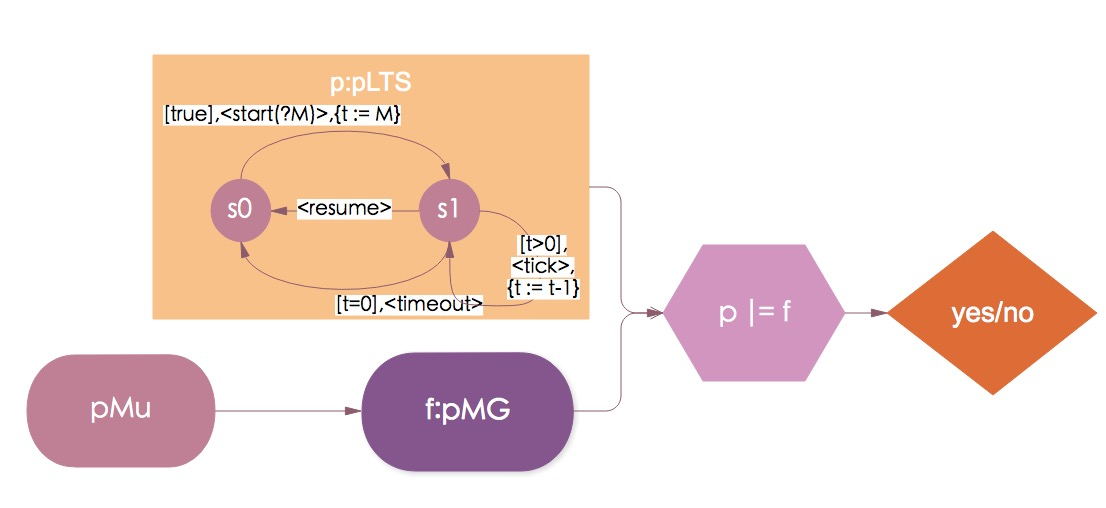
\includegraphics[width=5.5in]{figures/architectrue.jpeg} 
    \caption{Architecture of symbolic model checking}
    \label{architectrue}
\end{figure}




\subsection{Transformation from pM$\mu$ to pMG}


The transformation rules can be seen in Lin's paper~\cite{lin2001modal}. The rules take a pM$\mu$ formula as the input and generate a pMG. 

In the case study, the liveness property is present as Formula~\ref{formula1}. The alternation depth is 1, because there is only one $\mu$ operator. The corresponding modal graph is shown as follows:


\begin{figure}
	\begin{tikzpicture}[->, shorten >=2pt, >=stealth, node distance=2cm,
	noname/.style={ellipse, minimum width=2.5em, minimum height=1.5em, draw}]
	\node[noname] (1)                                            				 	{$t_{1}$};
	\node[noname] (2) [right=of 1]                               				 	{$t_{2}$};
	\node[noname] (3) [right=of 2]                              				 	{$t_{3}$};
	\node[noname] (4) [node distance=0.5cm and 2cm, above right=of 3]    {$t_{4}$};
	\node[noname] (5) [right=of 4]                                					{$t_{5}$};
	\node[noname] (6) [node distance=0.5cm and 2cm, below right=of 3]     {$t_{6}$};
	
	\path 	(1) edge                   	node[above] {} (2)
	(2) edge                   	node[above] {} (3)
	(3) edge 			node[above] {} (4)
	(3) edge 			node[above] {} (6)
	(6) edge[bend left]    node[below] {} (3)
	(4) edge    		node[below] {} (5);
	\end{tikzpicture}
	\caption{The associated pMG}
\end{figure}
where:
\begin{itemize}
	\item $L_{N}(t_{1}) = (\{\}, \langle start?M\rangle, 1)$
	\item $L_{N}(t_{2}) = (\{t\}, t := M, 1)$
	\item $L_{N}(t_{3}) = (\{t\}, \vee, 1)$
	\item $L_{N}(t_{4}) = (\{t\}, \langle timeout\rangle, 1)$
	\item $L_{N}(t_{5}) = (\{\}, true, 1)$
	\item $L_{N}(t_{6}) = (\{t\}, \langle tick\rangle, 1)$
\end{itemize}



\section{The algorithm}

\subsection{Background}

 In \cite{lin1996stga}, Lin presents a symbolic transition graph with assignment (STGA) to model concurrent processes. In a STGA, a node is associated with a set of variables. and the edge between nodes is labelled by guard, assignment and action with a tuple $(b, \bar{x}:=\bar{e}, \alpha)$. The first-order $\mu$-calculus is employed as the property language. In order to check the graph, the first-order $\mu$-calculus is transferred to a graphical version through the proposed rules, and then we check {\color{red}{STGA and the modal graph}} by the algorithm.
 

 
 \subsubsection{Parameterised action}
From the perspective of syntax, pLTS is similar to STGA. The difference between pLTS and STGA is the $\mathit{action}$. An action in pLTS is a parameterised action $c(args)$. From the syntax of pM$\mu$, we define the parameters in the action as $args$, and $args$ can be one of $!e$, $?x$ and $null$ or the composition of them. While an action in STGA is either a silent action $\tau$, an input action $c?x$, or an output action $c!e$, where $c\in Chan$. 

The difference in parameterised action results in the difference in modality of the algorithm. Based on similarity, we check the pLTS through modifying the algorithm, especially in the modality.  

\subsubsection{Alternation-free pM$\mu$}

A formula is said to be alternation-free, when the alternation depth is one, without mutually recursive greatest and least fixed-point operators. A formula expressed with pM$\mu$ is alternation-free. But the formula with first-order $\mu$-calculus have to deal with alternation depth.{\color{red}{[To do Tengfei: definition of alternation depth]}}


 {\color{red}{The order of action and conditional expression???}}
Another difference is the order of action and conditional expression. In pLTS, the order is $<\alpha, e_{b}, (x_{j}:=e_{j})^{j\in J}>$,  and $vars(e_{b})\subseteq vars(s)\cup vars(\alpha)$, and $\forall j\in J. vars(e_{j})\subseteq vars(s)\wedge x_{j}\in vars(s')$. 

While it is $< b, \bar{x}=\bar{e}, \alpha>$ in STGA.


\subsection{Abstract data domain}

In a pLTS, the parameterised action $start(?M)$ includes a parameter in it, and whether the parameter is a variable or a constant is unknown at the abstract level. Abstract values are associated with parameters instead of concrete values \cite{cousot1976static}. We use a symbolic interpretation on parameters $M$. 


{\color{red}{
To to Eric:
In order to construct the abstract data domains, we divide the value of $Max$ to variable and constant. If Max is a variable, Max can express the interval on integer. The change of the value is controlled by a self-decreasing operator. Also, we need another integer 0 as the minimal boundary. If Max is a constant, i.e. Max is the maximal boundary and 0 is the minimal boundary. So we need another variable $pos$ as the interval between Max and 0. Fig.~\ref{side:a} and Fig.~\ref{side:b} are two interpretations on the data domain of the variables. Fig.~\ref{side:a} shows an interpretation that includes two constant (Max, 0), a variable (pos) and an operator (-) on the integer. While Fig.~\ref{side:b} specifies that $Max$ is a variable.
}}


\begin{figure}[htbp]

	\begin{tikzpicture}[->, shorten >=2pt, >=stealth, node distance=1.5cm,
	noname/.style={ellipse, minimum width=2.5em, minimum height=1.5em,draw}]
	\node[noname] (1)                                             {$Max$};
	\node[noname] (2) [node distance=0.5cm and 2cm, above right=of 1]                                {$0$};
	\node[noname] (3) [node distance=0.5cm and 2cm, below right=of 1]                                {$pos$};
	
	\path 	(1) edge                   	node[above] {$-$} (2)
	(1) edge                   	node[above] {$-$} (3)
	(3) edge                   node[right] {$-$} (2);
	\path[->] (3) edge [in=-10,out=20,loop] coordinate[pos=0.52] (midp) node[right] {$-$} (3);
	\end{tikzpicture}
	\caption{Interpretation on $Max$}   \label{side:a}

\end{figure}



\subsection{The algorithm for checking pLTS}


\subsubsection{Processing parameterised action}
We change the algorithm to make it suitable for checking pLTS. From the syntax of pM$\mu$, we define the parameters in the action as $args$, and $args$ can be one of $!e$, $?x$ and $null$ or the composition of them. In the modification version, we change the modality $[c!e], \langle c!e\rangle$, $[c?x], \langle c?x\rangle$ to $[c]$, $\langle c\rangle$, $[c(args)], \langle c(args)\rangle$.
It was shown as follows:

$[c]\Rightarrow$ $checkAnd(\{ (p_{i}, (n', \rho))\,|\, p \xrightarrow{c} p_{i}, n\rightarrow n' \})$
		
$\langle c\rangle\Rightarrow$ 
	 $checkOr(\{ (p_{i}, (n',\rho))\,|, p \xrightarrow{c} p_{i}, n \rightarrow n'\})$
		
$[c(?x, !e)]\Rightarrow$
	$ checkAnd(\{ (p_{i}[v/y], (n',\rho\{x \rightarrow v\}))\,|\,  n \rightarrow n', p \xrightarrow{c(?y, !\rho(e)) } p_{i},v\in Val\})$
		
{$\langle c(?x, !e)\rangle\Rightarrow$}
	 $ checkOr(\{ (p_{i}[v/y], (n', \rho\{x \rightarrow v\}))\,|\,  n \rightarrow n', p \xrightarrow{c(?y, !\rho(e))} p_{i},v\in Val\})$
		
The full algorithm can be seen in the appendix.

\subsubsection{Processing alternation-free pM$\mu$}
The formula in pM$\mu$ is alternation-free, so the alternation depth is 1 in each node of pMG. In the model checking graph, we don't need to use recursion, and the function $restore(D, b)$ in the algorithm is useless for checking pLTS.

{\color{red}{[The principle of model checking]}}
Given a pLTS model $M$ and a pMG formula $f$, the algorithm checks whether the model satisfies the formula $M\models f$. Each state is made up with a couple $\{s\rho, n\rho'\}$, where $s$ is a state in pLTS, and $n$ a node of pMG. A transition of the model checking graph is from $\{s\rho, n\rho_{0}\}$ to $\{s'\rho', n'\rho_{0}'\}$. 



\subsection{The execution result}

After running the algorithm in the appendix, the model checking graph is shown in Fig.~\ref{checkinggraph}:


\begin{figure}
	\begin{tikzpicture}[->, shorten >=2pt, >=stealth, node distance=2cm,
	noname/.style={ellipse, minimum width=3em, minimum height=1.5em, draw}]
	\node[noname] (1)                                             {$S_{0}$};
	\node[noname] (10) [node distance=0.5cm and 2cm, above right=of 1]                                {$S_{10}$};
	\node[noname] (11) [node distance=0.5cm and 2cm, below right=of 1]                                {$S_{11}$};
	\node[noname] (20) [node distance=0.5cm and 2cm, above right=of 10]                                {$S_{20}$};
	\node[noname] (30) [node distance=0.5cm and 2cm, above right=of 20]                                {$S_{30}$};
	\node[noname] (31) [node distance=0.5cm and 2cm, below right=of 20]                                {$S_{31}$};
	\node[noname] (40) [right=of 30]                                {$S_{40}$};
	
	
	\node[noname] (21) [node distance=0.5cm and 2cm, below right=of 11]                                {$S_{21}$};
	\node[noname] (32) [node distance=0.5cm and 2cm, above right=of 21]                                {$S_{32}$};
	\node[noname] (33) [node distance=0.5cm and 2cm, below right=of 21]                                {$S_{33}$};
	\node[noname] (41) [right=of 32]                                {$S_{41}$};
	
	
	\path 	(1) edge                   	node[above] {$\langle start?M\rangle,1$} (10)
	(1) edge                   	node[above] {$\langle start?M\rangle,1$} (11)
	(10) edge                   node[above] {${\mu},1$} (20)
	(20) edge                 	node[above] {$\vee,1$} (30)
	(20) edge                 	node[above] {$\vee,1$} (31)
	(31) edge [bend left] 			node[below] {$\langle true\rangle,1$} (20)
	(30) edge               	node[above] {$\langle timeout\rangle,1$} (40)
	
	
	(11) edge                   node[above] {${\mu},1$} (21)
	(21) edge                 	node[above] {$\vee,1$} (32)
	(21) edge                 	node[above] {$\vee,1$} (33)
	(33) edge [bend left] 			node[below] {$\langle true\rangle,1$} (21)
	(32) edge               	node[above] {$\langle timeout\rangle,1$} (41);
	
	\end{tikzpicture}
	\caption{Model checking Graph}
	\label{checkinggraph}
\end{figure}
where:
\begin{itemize}
	\item $S_{0}  = (\{s_{0},s_{[\rho=\emptyset]}\}, \{n_{1}, \rho_{0}'=\emptyset\}\;|\;s.\sigma = false)$
	\item $S_{10} = (\{s_{1},s_{[t\leftarrow 0]}\}, \{n_{2}, \rho_{0}'(M\leftarrow 0)\}\;|\;s.\sigma = false)$
	\item $S_{20} = (\{s_{1},s_{[t\leftarrow pos]}\}, \{n_{3}, \rho_{0}'(t\leftarrow n_{2})\}\;|\;s.\sigma = false)$
	\item $S_{30} = (\{s_{1},s_{[t\leftarrow 0]}\}, \{n_{4}, \rho_{0}'(t\leftarrow 0)\}\;|\;s.\sigma = false)$
	\item $S_{31} = (\{s_{1},s_{[t\leftarrow 0]}\}, \{n_{5}, \rho_{0}'(t\leftarrow 0)\}\;|\;s.\sigma = false)$
	\item $S_{40} = (\{s_{0},s_{\rho[true]}\}, \{n_{6}, \rho_{0}'(true)\}\;|\;s.\sigma = true)$
	
	\item $S_{11} = (\{s_{1},s_{[t\leftarrow pos]}\}, \{n_{2}, \rho_{0}'(M\leftarrow pos)\}\;|\;s.\sigma = false)$
	\item $S_{21} = (\{s_{1},s_{[t\leftarrow pos]}\}, \{n_{3}, \rho_{0}'(t\leftarrow n_{2})\}\;|\;s.\sigma = false)$
	\item $S_{32} = (\{s_{1},s_{[t\leftarrow 0]}\}, \{n_{4}, \rho_{0}'(t\leftarrow 0)\}\;|\;s.\sigma = false)$
	\item $S_{33} = (\{s_{1},s_{\rho[t\leftarrow t-1]}\}, \{n_{5}, \rho_{0}'(t\leftarrow t-1)\}\;|\;s.\sigma = false)$
	\item $S_{41} = (\{s_{0},s_{\rho[true]}\}, \{n_{6}, \rho_{0}'(true)\}\;|\;s.\sigma = true)$
	\item $n_{2}'=\mu X(pos/t)(\langle timeout\rangle true \vee \langle true\rangle X(pos-1))$
	\item $n_{3}=\langle timeout\rangle true \vee\langle true\rangle\mu X(pos)(\langle timeout\rangle true \vee \langle true\rangle X(pos-1))$
\end{itemize}

In the initial state, there is no variable for the pLTS. After the action $start(?M)$ triggers the transition from $s_{0}$ to $s_{1}$, the value of the variable $t$ will be changed to $Max$. In the transition, the action expression of the operator in the edge of pMG will trigger the occurrence of transitions in pLTS. The change of value in $s$ depends on the semantics of pLTS. In the state $s_{1}$, the system will check whether the guard $t>0$ satisfies. If yes, the action $tick$ will lead to the occurrence of loop transition. Or, the system will enter another transition back to the initial state $s_{0}$. {\color{red}{[After executing the model checking graph, it will finally return to state $S_{40}$ or state $S_{41}$. Both of them are true.}}



\section{Checking open automata}

\subsection{The difference between pLTS and open automata}

\subsection{}

\subsection{}



\section{Related work and Conclusion}



\section*{Appendix}

\algnewcommand\algorithmicswitch{\textbf{switch}}
\algnewcommand\algorithmiccase{\textbf{case}}
\algnewcommand\algorithmicassert{\texttt{assert}}
\algnewcommand\Assert[1]{\State \algorithmicassert(#1)}%
% New "environments"
\algdef{SE}[SWITCH]{Switch}{EndSwitch}[1]{\algorithmicswitch\ #1\ \algorithmicdo}{\algorithmicend\ \algorithmicswitch}%
\algdef{SE}[CASE]{Case}{EndCase}[1]{\algorithmiccase\ #1}{\algorithmicend\ \algorithmiccase}%
\algtext*{EndSwitch}%
\algtext*{EndCase}%

\begin{algorithm} 
	\begin{algorithmic}[1]
		\State stack[0 ... (k-l)]
		\State pushStack(s) = push s onto stack[s.depth]
		\State top() = return the top element of the first non-empty stack with the deepest depth
		\State pop() = remove from the stack the element returned by the last call to top 
		\State $s=\{s.depth, s.status, s.\sigma, s.D, s.instack\}$
		\State modelCheck(s) = \{ s.status := VISITED($s.\sigma)$; push(s);
		\While{stack is non-empty}
		\State close(top()); \Return s.status; \}
		\EndWhile
		
	\end{algorithmic} 
	\caption{modelCheck(s)}
	\label{alg:algorithm1}
\end{algorithm}

\begin{algorithm} 
	\begin{algorithmic}[1]
		
		\State close(s as ($p, n\rho'$)) =
		\If{n is root}
		\State $p = m\rho; \rho = \emptyset; \rho' = \emptyset$  
		\EndIf
		\State let checkAnd(W) =
		\State let ($B_{i}, D_{i}$) = check($s_{i}$) 
		\For {each $s_{i} \in W$}
		\If {there is some $B_{i}$ = DEFERRED}
		\Return(DEFERRED)
		\ElsIf {there is some $B_{i}$ = VALUE(false)} 
		\State add s to $D_{i}$; \Return(VALUE(false))
		\Else 
		\State add s to each $D_{i}$; \Return(VALUE(true))
		\EndIf
		\EndFor
		\State let checkOr(W) =
		\State let ($B_{i}, D_{i}$) = check($s_{i}$) 
		\For {each $s_{i} \in W$}
		\If {every $B_{i}$ = DEFERRED}
		\Return(DEFERRED)
		\ElsIf{there is some $B_{i}$ = VALUE(true)} 
		\State add s to $D_{i}$; \Return(VALUE(true))
		\Else 
		\State add s to each $D_{i}$; \Return(VALUE(false))
		\EndIf
		\EndFor
		
		
		\State  let $B$ be 
		\Switch{$L_{O}(n)$} 
		\Case{$be$}
		\Return $\rho(be)$
		\EndCase
		\Case{x:=e}
		\Return $checkAnd(\{ (p, (n', \rho\{x\rightarrow \rho(e)\}))\, |\, n \rightarrow n' \})$
		\EndCase
		\Case{$\wedge$} 
		\Return $checkAnd(\{ (p, (n_{i}, \rho))\, n\rightarrow n_{i}\}) $
		\EndCase
		\Case{$\vee$} 
		\Return $checkOr(\{ (p, (n_{i}, \rho))\, n\rightarrow n_{i} \})$
		\EndCase
		\Case{[c]} 
		\Return $checkAnd(\{ (p_{i}, (n', \rho))\,|\, p \xrightarrow{c} p_{i}, n\rightarrow n' \})$
		\EndCase
		\Case{$\langle c\rangle$} 
		\Return $checkOr(\{ (p_{i}, (n',\rho))\,|, p \xrightarrow{c} p_{i}, n \rightarrow n'\})$
		\EndCase
		\Case{[c(?x, !e)]}
		\Return $ checkAnd(\{ (p_{i}[v/y], (n',\rho\{x \rightarrow v\}))\,|\,  n \rightarrow n', p \xrightarrow{c(?y, !\rho(e)) } p_{i},v\in Val\})$
		\EndCase
		\Case{$\langle c(?x, !e)\rangle$}
		\Return $ checkOr(\{ (p_{i}[v/y], (n', \rho\{x \rightarrow v\}))\,|\,  n \rightarrow n', p \xrightarrow{c(?y, !\rho(e))} p_{i},v\in Val\})$
		\EndCase
		\Case{$\forall x$}
		\Return $  checkAnd(\{ (p, (n',\rho\{x \rightarrow v\}))\,|\, n \rightarrow n', v \in Val\})$
		\EndCase
		\Case{$\exists x$}
		\Return $ checkOr(\{ (p, (n',\rho\{x \rightarrow v\}))\,|\,  n \rightarrow n', v\in Val\})$
		\EndCase
		\EndSwitch
		
		\If{B=VALUE(b)}
		\State pop(); 
		\If{s.status = VISITED($b'$) and $b'\neq b$}
		\State s.status = VISITED($b$); 
		\EndIf
		\EndIf
	\end{algorithmic} 
	\caption{$close(s)$}
	\label{alg:algorithm1}
\end{algorithm}	


\begin{algorithm} 
	\begin{algorithmic}[1]
		\State check(s) =
		\Switch{$s.status$}
		\Case{FRESH} 
		\State s.status := VISITED($s.\sigma$); push($s$); \Return (DEFERRED, $s.D$)
		\EndCase
		\Case{VISITED($b$)} 
		\Return (VALUE($b$), $s.D$)
		\EndCase
		\EndSwitch
		
	\end{algorithmic} 
	\caption{check(s)}
	\label{alg:algorithm2}
\end{algorithm}





\begin{thebibliography}{4}
	
	\bibitem{radu2008mcl}Mateescu, Radu, and Damien Thivolle. "A model checking language for concurrent value-passing systems." International Symposium on Formal Methods. Springer, Berlin, Heidelberg, 2008.
	
	\bibitem{mavridou2016architectrue} Mavridou, Anastasia, et al. "Architecture-based design: A satellite on-board software case study." International Workshop on Formal Aspects of Component Software. Springer, Cham, 2016.
	\bibitem{lin2001modal} Lin, Huimin. "Model checking value-passing processes." apsec. IEEE, 2001.

	\bibitem{lin1996stga} Lin, Huimin. "Symbolic transition graph with assignment." International Conference on Concurrency Theory. Springer, Berlin, Heidelberg, 1996.
	\bibitem{cousot1976static}Cousot, Patrick, and Radhia Cousot. "Static determination of dynamic properties of programs." Proceedings of the 2nd International Symposium on Programming, Paris, France. Dunod, 1976.
	
\end{thebibliography}




\end{document}
